%==============================================================================
% Sjabloon onderzoeksvoorstel bachproef
%==============================================================================
% Gebaseerd op document class `hogent-article'
% zie <https://github.com/HoGentTIN/latex-hogent-article>

\documentclass{hogent-article}

% Invoegen bibliografiebestand
\usepackage[backend=biber,style=apa]{biblatex}
\DeclareLanguageMapping{dutch}{dutch-apa}
\addbibresource{voorstel.bib}

% Informatie over de opleiding, het vak en soort opdracht
\studyprogramme{Professionele bachelor toegepaste informatica}
\course{Bachelorproef}
\assignmenttype{Onderzoeksvoorstel}

\academicyear{2023-2024}

% TODO: Werktitel - nog aan te passen
\title{Gamification om werknemers aan het sporten te krijgen}

\author{Sarah Eggermont}
\email{sarah.eggermont@student.hogent.be}


% TODO: Geef de co-promotor op - meerdere?
\supervisor[Co-promotor]{G. Vande Maele (we are, \href{mailto:guillaume@we-are.be}{guillaume@we-are.be})}
\supervisor[Co-promotor]{M. De Buck (we are, \href{mailto:manu@we-are.be}{manu@we-are.be})}

% Binnen welke specialisatierichting uit 3TI situeert dit onderzoek zich?
% Kies uit deze lijst:
%
% - Mobile \& Enterprise development
% - AI \& Data Engineering
% - Functional \& Business Analysis
% - System \& Network Administrator
% - Mainframe Expert
% - Als het onderzoek niet past binnen een van deze domeinen specifieer je deze
%   zelf
%
\specialisation{Mobile \& Enterprise development}
% TODO: keywords aanvullen
\keywords{Gamification, responsive website}

\begin{document}

\begin{abstract}
  Hier schrijf je de samenvatting van je voorstel, als een doorlopende tekst van één paragraaf. Let op: dit is geen inleiding, maar een samenvattende tekst van heel je voorstel met inleiding (voorstelling, kaderen thema), probleemstelling en centrale onderzoeksvraag, onderzoeksdoelstelling (wat zie je als het concrete resultaat van je bachelorproef?), voorgestelde methodologie, verwachte resultaten en meerwaarde van dit onderzoek (wat heeft de doelgroep aan het resultaat?).
\end{abstract}

\tableofcontents

% De hoofdtekst van het voorstel zit in een apart bestand, zodat het makkelijk
% kan opgenomen worden in de bijlagen van de bachelorproef zelf.
%---------- Inleiding ---------------------------------------------------------

\section{Introductie}%
\label{sec:introductie}

Een sedentaire job wordt geassocieerd met schadelijke gevolgen voor de algemene gezondheid \autocite{Buckley2015}. Het is dus van groot belang dat voldoende beweging een prioriteit is.

\textcite{Hallal2012} beschouwen 31,1\% van de wereldwijde bevolking als inactief. Dit wil zeggen dat, op het moment van onderzoek, bijna een derde van de volwassen wereldbevolking de vooropgestelde aanbevelingen van ``World Health \linebreak Organization'' (WHO), beschreven door \textcite{Bull2020}, niet haalt. Voor Europa ligt deze waarde zelfs op 34,8\% en zoals op Figuur \ref{fig:inactivity} te zien is, ligt België nog een stuk boven de gemiddelde Europese waarde met 40\% à 49,9\%.

\begin{figure}[t]
    \caption{Fysieke inactiviteit volwassenen (15+) wereldwijd, bij mannen (A) en vrouwen (B) \autocite{Bull2020}}
    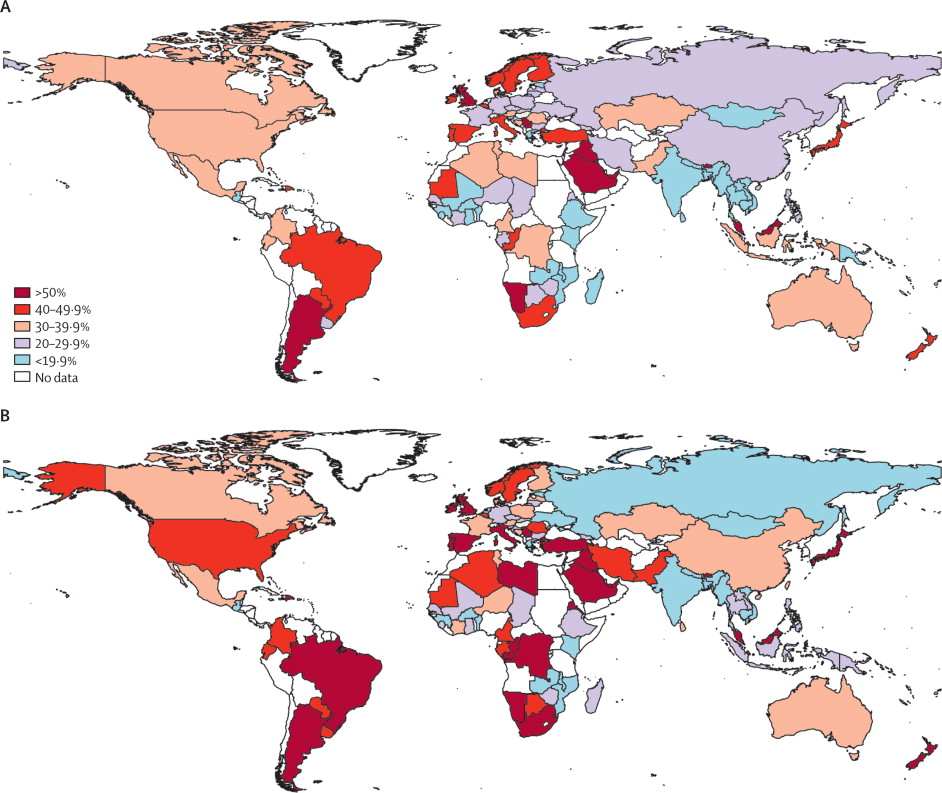
\includegraphics[width=0.5\textwidth]{Inactiviteit}
    \label{fig:inactivity}
\end{figure}

Om deze problematiek te proberen verhelpen, zal een sportplatform ontwikkeld worden. Deze paper onderzoekt hoe gamification hierbij kan helpen. Gamification is in de literatuur beschreven als het gebruiken van spelelementen in een context die niet aan een spel gerelateerd is \autocite{Gaalen2020}.

In de literatuurstudie zal allereerst het belang van voldoende beweging voor een goede gezondheid nog verder gekaderd worden. Daarna zal het effect van die beweging en gezonde levensstijl op productiviteit geïllustreerd worden. Vervolgens zal het concept van gamification diepgaander uiteengezet worden, door onder andere in te zoomen op de meest gebruikte technieken, de sociale en psychologische aspecten en de invloed op het gebruikersgedrag. Ten slotte wordt er gekeken naar bestaande sportapplicaties en -platformen, en beschreven welke vormen van gamification daar in voorkomen.

Nadien zal in de methodologie worden uiteengezet welke stappen er nodig zijn om tot het sportplatform te komen dat, door middel van gamification, werknemers van \textbf{bedrijfX} en \textbf{bedrijfY} motiveert om meer te sporten.

Uiteindelijk kunnen de conclusies van het onderzoek teruggevonden worden.


%---------- Stand van zaken ---------------------------------------------------

\section{Literatuurstudie}%
\label{sec:state-of-the-art}

\subsection{Belang van beweging}

Bij volwassenen wordt een sedentaire levensstijl geassocieerd met schadelijke gevolgen voor de volgende gezondheidskwesties: sterfte in het algemeen, sterfte door hart- en vaatziekten en kanker, het voorkomen van hart- en vaatziekten, diabetes type 2 en kanker \autocite{Bull2020}. Daarnaast gaat verminderde fysieke activiteit ook gepaard met meer depressie-, angst- en stresssymptomen \autocite{Stanton2020}.

Om de kans hierop te verkleinen moeten volwassenen, tussen de 18 en 64 jaar oud, volgens de WHO wekelijks 150 à 300 minuten sporten met gemiddelde intensiteit of 75 à 150 minuten met krachtige intensiteit \autocite{Bull2020}. Voor mensen met een beperking worden dezelfde hoeveelheden sport aangeraden, hoewel daar mogelijks samen met een medisch verantwoordelijke bekeken moet worden in welke mate dit mogelijk is, afhankelijk van de beperking. Voor zwangere of net bevallen vrouwen wordt er minstens 150 minuten per week, met gemiddelde intensiteit, aangeraden.

\subsection{Beweging en productiviteit}

Wanneer de algemene gezondheid van werknemers slecht is, brengt dit kosten mee voor het bedrijf. \textcite{Sjoegaard2016} beschrijven hoe deze kosten gerelateerd zijn aan de mentale en fysieke afwezigheid van werknemers tijdens het werk, met een verminderde productiviteit tot gevolg. Echter, voor personen die sedentair werk uitvoeren en voornamelijk aan een computer werken, zorgt een verhoogde hoeveelheid sport tijdens de vrije tijd voor minder stres en meer energie op de werkvloer \autocite{Hansen2009}. Op die manier leidt het invoeren van regelmatige beweging, door middel van op voorhand opgestelde oefeningen en een zorgvuldige begeleiding, volgens \textcite{Cancelliere2011} tot een positief effect op de productiviteit. In die mate dat \textcite{Sjoegaard2016} stellen dat dit effect de eventuele uitgaven in verband met sportactiviteiten overstijgen.

\subsection{Gamification}

Volgens \textcite{Deterding2011} is gamification te beschrijven als het gebruiken van speldesignelementen in een niet-spelgerelateerde context. Gamification bestaat uit drie hoofdonderdelen: de gebruikte techniek, de psychologische uitkomsten en de verdere invloed op het gedrag \autocite{Hamari2014}. Daarnaast zijn sociale aspecten ook essentieel: door het ontstaan van een competitie streven mensen ernaar erkenning te ontvangen \autocite{Hamari2013}.

\subsubsection{Meest gebruikte technieken}

\textcite{Hamari2014} somt punten, scoreborden en vooropgestelde uitdagingen op als de drie \linebreak meest voorkomende technieken. Daarnaast komen ook volgende methodes veelvuldig voor: het gebruik van levels, en eventueel een daarbij horend verhaal, beloningen, een overzicht van vooruitgang of het bekomen van badges, die bijvoorbeeld de beste gebruiker in een bepaalde categorie aanduiden \autocite{Dong2012,Flatla2011,Li2012}.
Daarbij kunnen de gehanteerde technieken verder ingevuld worden naar wens. Zo kunnen beloningen bijvoorbeeld bestaan uit, maar daarom niet gelimiteerd worden tot, een donatie aan een gekozen goed doel of een eervolle vermelding op een intern bedrijfsevenement.

\subsubsection{Sociale aspecten}

Er zijn twee belangrijke sociale aspecten om in acht te nemen wanneer gamification geïmplementeerd wordt.

Enerzijds is er erkenning, wat beschreven kan worden als de sociale feedback die gebruikers krijgen op hun gedrag \autocite{Cheung2011}.
Wanneer een dienst, zoals het aanbieden van een platform met gamification, erkenning van de andere gebruikers oplevert, wordt die dienst positiever ervaren \autocite{Preece2001}.
\textcite{Hamari2013} suggereren dat er vervolgens, als gevolg van de ontvangen erkenning, een bepaalde bereidheid ontstaat om de erkenning wederkerig te maken. Hierdoor zal de tegenpartij ook op zijn beurt de dienst positiever ervaren.

Anderzijds is er sociale invloed, wat verwijst naar de perceptie van een individu over het belang dat anderen hechten aan een bepaald doelgedrag en of ze verwachten dat iemand dat gedrag zal vertonen \autocite{Ajzen1991}. Specifiek voor een platform dat gamification implementeert, kan er sociale invloed ontstaan door het zien van wat andere gebruikers op het platform presteren. Hierdoor wordt namelijk een verwachtingspatroon gecreëerd en zetten gebruikers elkaar aan tot het behalen van een bepaald doelgedrag, zoals vaker sporten.

\subsubsection{Psychologische aspecten}

Wanneer psychologische gevolgen op de gebruiker bevraagd zijn, wordt er vooral gefocust op motivatie, attitude en plezier \autocite{Hamari2014}. \textcite{Cheong2013} werkte een online quiz uit die gamification gebruikt, met als doel om bijleren te motiveren en leuker te maken. Uit een bevraging  na de quiz bleek dat 40,79\% van de deelnemers enthousiast en 46,05\% van de deelnemers tevreden was tijdens de quiz. Daarenboven was het merendeel (77,63\%) van de deelnemers voldoende gemotiveerd om de quiz te vervolledigen.

\subsubsection{Invloed op gedrag}

\textcite{Kari2016} stellen dat gamification in sportapplicaties een positieve invloed heeft op de intrinsieke bewegingsmotivatie, wat ervoor zorgt dat gebruikers gaan handelen naar een bepaald doelgedrag. \textcite{PoloPena2020} bevestigen dit, maar voegen hier wel aan toe dat gamification een grotere invloed heeft op vrouwen dan op mannen, en op oudere mensen dan op jongere gebruikers.

Studies van \textcite{Hamari2013a} hebben aangetoond dat de resultaten van gamification mogelijks niet voor alle gebruikers op lange termijn doeltreffend zijn, en de invoering ervan mogelijks niet op iedereen het gewenste effect heeft.
Anderzijds zal het verwijderen van spelelementen uit een dienst schadelijke gevolgen voor de gebruikers hebben die wel nog betrokken zijn tot het gamification-aspect: zo kan een gebruiker plots al diens vooruitgang of verdiende badges verliezen.

\subsection{Bestaande sportapplicaties}

Hieronder volgt een diverse greep uit de bestaande mobiele en desktop sportapplicaties en -platformen en welke spelelementen daarin gebruikt worden.

\href{https://www.strava.com/}{Strava} is een applicatie waarmee gebruikers hun sportprestaties kunnen bijhouden. \textcite{Barratt2017} stelt dat deze applicatie gamification toepast, zoals uitdagingen en persoonlijke en trainingsvooruitgang.

\href{https://www.nike.com/be/en/nrc-app}{Nike Run Club} is een loopapplicatie met meer dan 10 miljoen downloads\footnote{\href{https://bootcamp.uxdesign.cc/how-the-nike-run-club-app-got-runners-hooked-2850c7654fc5}{How the Run Club App got runners hooked - Leevey}} op de Google Play Store en de App Store. Deze applicatie maakt het mogelijk voor lopers om een looptraining vast te leggen, punten te verdienen en andere gebruikers uit te dagen. Daarnaast kunnen ze eigen doelstellingen aanmaken en delen, zodat samen naar een gezamenlijk doel gewerkt kan worden \autocite{StaalnackeLarsson2013}.

Een derde voorbeeld is \href{https://connect.garmin.com/}{Garmin Connect}. Het verschil met de vorige twee applicaties is dat dit platform enkel voor gebruikers met een Garmin-toestel bedoeld is. Deze applicatie focust vooral op badges \autocite{Ilhan2019}. Het behalen van zulke badge kan dan punten opleveren en de mogelijkheid geven tot het behalen van nieuwe, meer uitdagende badges. Om negatieve gevoelens van frustratie op een mindere dag tegen te gaan, krijgt de gebruiker de optie om andere, niet fysieke activiteiten uit te voeren om ook dan punten te verdienen.

Een platform dat aan de criteria van deze casus voldoet, bestaat nog niet en zal dus ontwikkeld moeten worden in een volgende fase van het onderzoek.


%---------- Methodologie ------------------------------------------------------
\section{Methodologie}
\label{sec:methodologie}

Het onderzoek zal beginnen met een literatuurstudie die het belang van voldoende beweging kadert, vervolgens bespreekt wat het effect hiervan is op productiviteit en tenslotte gamification verder uitdiept. Het is bij dit laatstse belangrijk om technieken te identificeren die van toepassing zijn op deze specifieke casus. De resultaten hiervan kunnen gebruikt worden in de volgende fase.

Deze volgende fase bestaat uit een bevraging bij IT-werknemers van \textbf{bedrijfX} en \textbf{bedrijfY}. De bedoeling hiervan is enerzijds achterhalen in \linebreak welke mate sport en beweging een rol speelt in hun dagelijkse leven op het moment van het interview, en anderzijds te weten komen in welke mate en op welke manieren deze werknemers gestimuleerd kunnen worden om meer te gaan sporten, aan de hand van een competitief sportplatform. Hier kan ook de theorie die verkregen is uit de literatuurstudie getoetst worden.

Steunend op de bekomen resultaten uit zowel de literatuurstudie als de analyse van de gebruikersinterviews, zal dan een applicatie ontwikkeld worden. Het platform zal bestaan in de vorm van een responsive website, waarin sportgegevens van deelnemende werknemers worden verzameld aan de hand van applicaties en hun ''Application Programming Interface'' (API) zoals \linebreak \href{https://developers.strava.com/}{Strava}, \href{https://dev.fitbit.com/}{Fitbit} en \href{https://developer.garmin.com/gc-developer-program/overview/}{Garmin Connect}. Deze gegevens zullen in combinatie met gamification gebruikt worden om een competitie tussen de deelnemende bedrijven op te zetten.

Deze POC zal dan dienen om de hypotheses te toetsen: heeft het competitief sportplatform, dat gebruik maakt van gamification, een positieve invloed op het sportgedrag van werknemers in een sedentaire job? Om deze vraag te beantwoorden zullen opnieuw gebruikersinterviews plaatsvinden, met dezelfde personen die voor aanvang van de ontwikkelingsfase geïnterviewd zijn en die voor een periode van enkele weken deze POC hebben kunnen gebruiken. Een grondige analyse van de sportgegevens op het platform en de antwoorden van deze ondervraging, leiden tot de conclusie van dit onderzoek.


%---------- Verwachte resultaten ----------------------------------------------
\section{Verwacht resultaat}%
\label{sec:verwachte_resultaten}

De verworven kennis geeft momenteel aan dat een sportplatform met implementatie van gamification wel degelijk een positieve invloed zal hebben op het sportgedrag van gebruikers. Het verwachtte resultaat gaat er van uit dat er voldoende aandacht besteed wordt aan het sociale aspect van gamification en dat de gebruikers ook hun persoonlijke ontwikkeling en groei kunnen opmerken op het platform.

Ten gevolge van de positieve invloed op het sportgedrag van de deelnemende bedrijven, \linebreak wordt ook minder stress en een verbeterde productiviteit en tevredenheid op de werkvloer verwacht.

\printbibliography[heading=bibintoc]

\end{document}